% !TEX TS-program = xelatex
% !TEX encoding = UTF-8 Unicode
% !Mode:: "TeX:UTF-8"

\documentclass{resume}
\usepackage{zh_CN-Adobefonts_external} % Simplified Chinese Support using external fonts (./fonts/zh_CN-Adobe/)
% \usepackage{NotoSansSC_external}
\usepackage{NotoSerifCJKsc_external}
% \usepackage{zh_CN-Adobefonts_internal} % Simplified Chinese Support using system fonts
\usepackage{linespacing_fix} % disable extra space before next section
\usepackage{cite}
\usepackage{graphicx}
\usepackage{tabu}
\usepackage{multirow}
\usepackage{progressbar}

\begin{document}
\pagenumbering{gobble} % suppress displaying page number

\begin{center}
\Huge{个~~~人~~~简~~~历}
\end{center}
\\
\Large{
  \begin{tabu}{ c l l }
   \multirow{5}{1in}{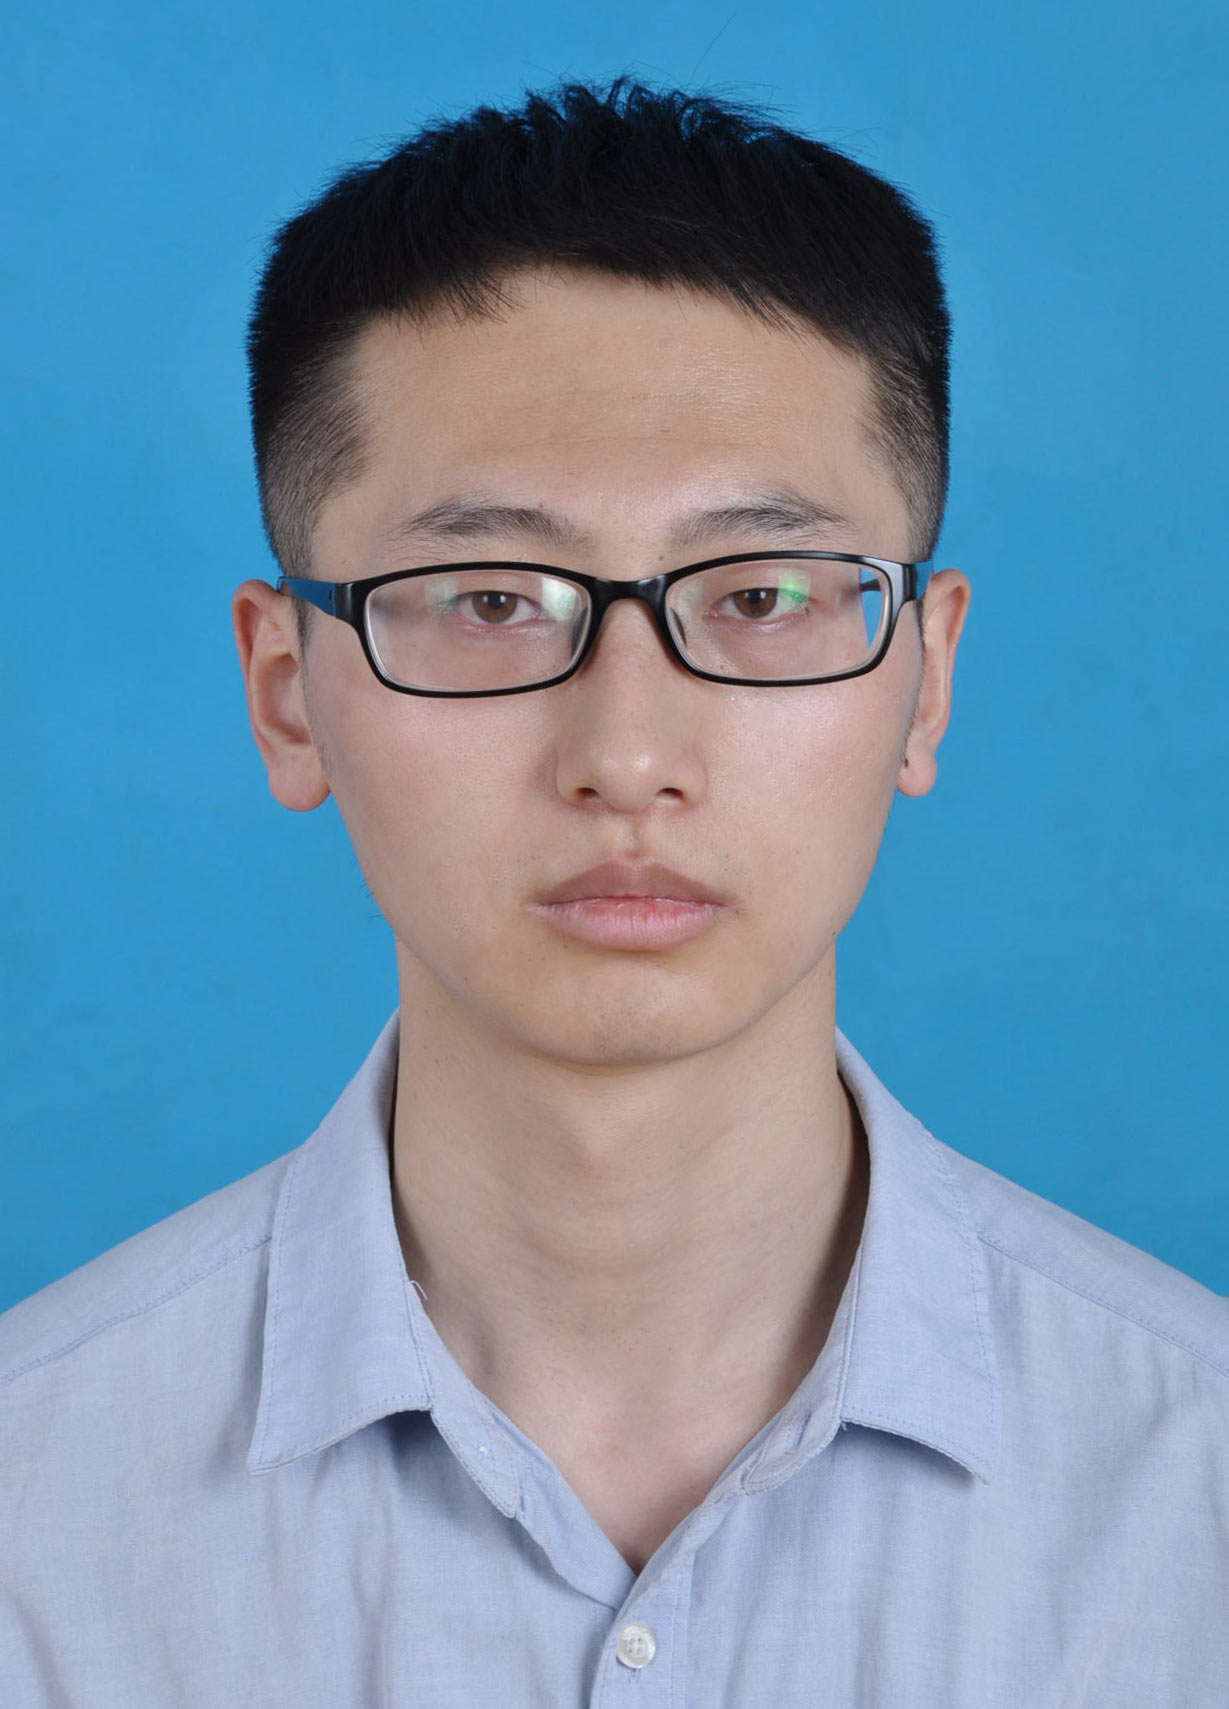
\includegraphics[width=0.88in]{avatar}} &
   \scshape{李高阳} &  \\
    & 性别:男 & 民族:汉 \\
    & 电话:(+86) 15002555080 & 生日:1995-09 \\
    & 邮箱:li.gaoyang@foxmail.com & 微信:sandbox\_ligy\\
    % & 地址:甘肃省兰州市天水南路222号 \hspace{40} & %籍贯:甘肃宁县
    & 个人主页:https://github.com/GoldenRaven & 政治面貌:党员
  \end{tabu}
}

\section{教育经历}
% \textbf{兰州大学}
\datedsubsection{\textbf{兰州大学\ 硕博连读与中科院兰州近物所联合培养博士}}{2013 -- 2019}
\textit{专业:物理学$\cdot$ 理论物理}\\
\textit{方向:凝聚态理论数值计算方法}
% \textit{导师:罗洪刚教授(长江学者)、房铁峰教授}\\
% \textit{研究内容:强关联量子系统的数值重整化群研究}\\
% \textit{研究方法:全密度矩阵数值重整化群(数值方法)}
\datedsubsection{\textbf{兰州大学\ 本科}}{2009 --  2013}
\textit{专业:物理学国家基地班\ \ 理论物理}

\section{发表文章}
\begin{itemize}
\item \textbf{Gao-Yang Li}, Tie-Feng Fang, Ai-Min Guo, and Qing-Feng Sun \textit{Ferromagnetism-induced Kondo effect in graphene with a magnetic impurity}, Phys. Rev. B \textbf{100}, 115115 (2019).
\item Wan-Xiu He, Zhan Cao, \textbf{Gao-Yang Li}, Lin Li, Hai-Feng Lü, ZhenHua Li, and Hong-Gang Luo \textit{Performance of the T-matrix based master equation for Coulomb drag in double quantum dots}, Phys. Rev. B \textbf{101}, 035417 (2020).
\end{itemize}

\section{获奖情况}
\datedline{\textit{国家励志奖学金}}{2010 -- 2011}
\datedline{\textit{学校三等奖学金}}{2013 -- 2018}
% \datedline{其他奖项}{2015}

\section{项目经验}
\begin{itemize}%[parsep=0.5ex]

\item \datedline{\textbf{{基于FORTRAN实现了模拟退火算法}}}{\textbf{{2014/08 -- 2014/10}}}
\textbf{项目描述}:导师基于对学术问题的认识提出了猜测函数,对其波函数作变分优化即可得到基态,进而研究其相变。 对于这个没有明确函数表达式的最小值优化问题,需要用数值方法在大参数范围内得到其稳定的最小值。\\
\textbf{职责描述}:用Fortran实现了模拟退火算法,设计了针对此问题的优化策略,并在感兴趣的参数范围内对程序进行了调试,在求解Rabi 模型的应用中取得了较好的结果。

% \item  \datedline{\textbf{{用HEOM程序研究了双量子点中的库仑drag效应}}}{\textbf{{2014/10 -- 2015/10}}}
% \textbf{项目描述}:在双量子点系统中的一个量子点电极两端施加电压,会在与之耦合的另一个量子点电极两端诱导出电流,我们想要研究这一效应的的物理机制。HEOM程序是近几年发展的新方法,是少数能研究非平衡双量子点系统的数值方法之一。程序由Fortran语言写成,体量在八千行左右,要使用大量内存,硬盘及高性能CPU。我们使用HEOM程序对双量子点系统进行了研究,成果发表在SCI二区期刊PRB上。\\
% \textbf{职责描述}:用时一周出差学习了HEOM程序,并在项目中负责提供集群脚本、程序调试、数据初期处理等。

\item \datedline{\textbf{{基于C++实现了数值重整化群程序}}}{\textbf{{2015/10 -- 2019/12}}}
{\textbf{项目描述}:数值重整化群程序是本领域中求解量子杂质问题最可靠的大型程序,其中涉及自洽迭代、消除累积误差、矩阵乘法、矩阵截断、稠密矩阵对⻆化等矩阵向量操作。实现中调用了 Intel MKL 库,并作了单节点 OpenMP 并行优化。本程序克服了老算法上的一些缺陷,并将精度由传统的97\%提高到99.9\%,部分研究成果整理成了学术论文,发表在SCI二区期刊PRB上。}\\
\textbf{职责描述}:独立完成了算法的调研、公式推导、程序结构的设计、程序的编写及优化,并完成后续对物理问题的探索与总结。程序总体量三千多行,运行时需占用内存约12GB。

% \textbf{职责描述}:完成了对数据集的清洗、特征组合,训练了SVM, DecisionTree, RandomForest, AdaBoost, GradientBoost 等模型并用投票集成对结果进行了改进,最后作了数据可视化。
% \item \datedline{\textbf{{基于Scikit-Learn实现了对MNIST数据集的分类}}}{\textbf{{2020/02 -- 至今}}}
% \textbf{项目描述}:对于MNIST手写数字数据集,训练得到一个能以较高精度对手写数字进行识别的KNN模型。\\
% \textbf{职责描述}:完成了数据可视化、模型训练、交叉验证以及超参调优,并在原数据集上做了数据集增广,使模型表现更好。

\item \datedline{\textbf{{实现了完整的机器学习项目流程}}}{\textbf{{2020/02 -- 至今}}}
\textbf{项目描述}:基于sklearn库,在房价数据集、泰坦尼克号等数据集上完成了对数据集的清洗、特征组合,训练了逻辑回归, SVM, 随机森林, 梯度提升树 等模型并用投票集成对结果进行了改进,预测的准确率达到较高水平,最后作了数据可视化,完成了完整的机器学习项目。

\item \datedline{\textbf{{针对商业银行信用卡业务的评分卡建模}}}{\textbf{{2020/02 -- 至今}}}
利用credit crisis数据集中用户的贷款、违约、教育程度、家庭等信息数据,经过数据清理、数据分箱、变量筛选等步骤,使用Logistic回归模型,建立了评分卡模型,并用ROC AUC来衡量模型的性能,最终按用户的模型得分划定了用户的信用等级。

\item \datedline{\textbf{{神经网络的分布式并行训练}}}{\textbf{{2020/02 -- 至今}}}
基于Pytorch库用ResNet实现了Cifar10图像数据集的分类;用AutoEncoder算法实现了图片的降噪;训练了卷积生成对抗网络DCGAN来生成新的“手写”数字。在两个节点共8个GPU上实现了Pytorch的分布式并行训练,大大缩短了训练时间。

% \item \textbf{数据挖掘}\\
% 学习了整个数据挖掘流程,包括了数据的获取、数据解析、数据评估、探索性数据分析、数据清理、特征工程、机器学习建模、模型评估以及结论可视化等。实现了基于sklearn的消费顾客群体聚类分析、谷歌应用商店APP数据使用量分析等。

% \item \textbf{深度学习算法}\\
% 学习了常用的深度学习算法,如简单神经网络、卷积神经网络、循环神经网络、自动编码器、对抗生成网络等。;用LSTM进行了烂番茄网站电影评论的情感分析。

\end{itemize}

\section{其他技能}
% increase linespacing [parsep=0.5ex]
\begin{itemize}%[parsep=0.5ex]
\item 熟悉常用机器学习算法如SVM, GradientBoosting, PCA, 层次聚类等,有深度学习算法如CNN, ResNet, AE, GAN, DCGAN的使用经验
%% \item 在Linux平台上配置了Pytorch并行CUDA环境,并利用两个节点共八个GPU进行了分布式并行加速
% \item 有Numpy, Scipy, Pandas, Scikit-Learn, Matplotlib等的使用经验
\item 能高效使用Shell脚本,有六年的Linux, Emacs, Git使用经验
\item 英语六级,能流利进行口头交流
% \item 平常编写代码要求尽量高效、美观,并用git管理代码
% \item 自学能力强,对新知识有较高的学习热情,并能投入精力解决问题
% \item 自学了机器学习的基本知识
% \item 了解精确对角化、密度矩阵重整化群、蒙特卡罗、张量网络重整化群等数值计算方法
% \item 喜欢打羽毛球
\item 本科学习成绩在本专业前30\%
\end{itemize}

\section{自我评价}
\qquad 自认为是一个上进努力有责任心的人,能和周围的人和睦相处,进行高效的交流。自学能力强,对新知识有较高的学习热情,能够以需求为导向,自驱地学习需要的知识,并能投入精力解决问题。

% \section{个人主页}
% \rm{https://github.com/GoldenRaven}

%% Reference
% \newpage
% \bibliographystyle{IEEETran} \bibliography{mycite}
\end{document}
